\section{Introduction}
\label{sec:nn-calibration:introduction}

Recent advances in deep learning have dramatically improved neural network accuracy \citep{simonyan2014very, srivastava2015highway, he2015deep, huang2016deep, huang2016densely}.
As a result, neural networks are now entrusted with making complex decisions in applications, such as object detection \cite{girshick2015fast}, speech recognition \cite{hannun2014deep}, and medical diagnosis \cite{caruana2015intelligible}.
In these settings, neural networks are an essential component of larger decision making pipelines.

%In real-world decision making systems, classification networks must not only be accurate, but also should indicate when they are likely to be incorrect.
%As an example, consider a self-driving car that uses a neural network to detect pedestrians and other obstructions \cite{bojarski2016end}.
%If the detection network is not able to confidently predict the presence or absence of immediate obstructions, the car should rely more on the output of other sensors for braking.
%Alternatively, in automated health care, control should be passed on to human doctors when the confidence of a disease diagnosis network is low  \cite{jiang2012calibrating}.
%Specifically, a network should provide a \emph{calibrated confidence} measure in addition to its prediction.
%In other words, the probability associated with the predicted class label should reflect its ground truth correctness likelihood.

%\begin{figure}[t!]
	%\centering
	%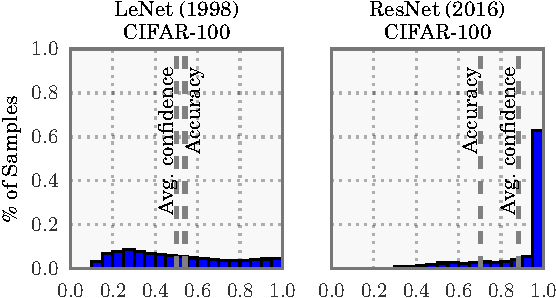
\includegraphics[width=0.8\columnwidth]{chapters/nn-calibration/figures/confidence.pdf}
	%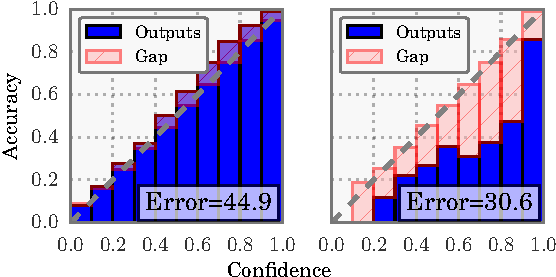
\includegraphics[width=0.8\columnwidth]{chapters/nn-calibration/figures/comparison_with_caruana.pdf}
	%\caption{Confidence histograms (top) and reliability diagrams (bottom) for a 5-layer LeNet (left) and a 110-layer ResNet (right) on CIFAR-100. Refer to the text below for detailed illustration.}
	%\label{figure.complenet}
	%\vspace{8pt}
%\end{figure}

%Calibrated confidence estimates are also important for model interpretability. Humans have a natural cognitive intuition for probabilities \cite{cosmides1996humans}. Good confidence estimates provide a valuable extra bit of information to establish trustworthiness with the user -- especially for neural networks, whose classification decisions are often difficult to interpret.
%Further, good probability estimates can be used to incorporate neural networks into other probabilistic models. For example, one can improve performance by combining network outputs with a language model in speech recognition \cite{hannun2014deep,xiong2016achieving}, or with camera information for object detection \citep{kendall2015modelling}.

In 2005, \citet{niculescu2005predicting} showed that neural networks typically produce well-calibrated probabilities on binary classification tasks. While neural networks today are undoubtedly more accurate than they were a decade ago,
we discover with great surprise that \emph{modern neural networks are no longer well-calibrated}.
This is visualized in \autoref{figure.complenet}, which compares a 5-layer LeNet (left) \cite{lecun1998gradient} with a 110-layer ResNet (right) \cite{he2015deep} on the CIFAR-100 dataset.
The top row shows the distribution of prediction confidence (i.e. probabilities associated with the predicted label) as histograms.
The average confidence of LeNet closely matches its accuracy, while the average confidence of the ResNet is substantially higher than its accuracy.
% That is, the ResNet is \emph{severely overconfident}.
This is further illustrated in the bottom row reliability diagrams \cite{degroot1983comparison,niculescu2005predicting}, which show accuracy as a function of confidence. We see that LeNet is well-calibrated, as confidence closely approximates the expected accuracy (i.e. the bars align roughly along the diagonal). On the other hand, the ResNet's accuracy is better, but does not match its confidence.

% In this paper, we thoroughly study the problem of calibrating modern neural networks in supervised classification settings.
Our goal is not only to understand why neural networks have become miscalibrated, but also to identify what methods can alleviate this problem.
%
In this paper, we demonstrate on several computer vision and NLP tasks that neural networks produce confidences that do not represent true probabilities.
%
Additionally, we offer insight and intuition into network training and architectural trends that may cause miscalibration.
%
Finally, we compare various post-processing calibration methods on state-of-the-art neural networks, and introduce several extensions of our own. Surprisingly, we find that a single-parameter variant of Platt scaling \cite{platt1999probabilistic} -- which we refer to as \emph{temperature scaling} -- is often the most effective method at obtaining calibrated probabilities. Because this method is straightforward to implement with existing deep learning frameworks, it can be easily adopted in practical settings.
%
